% !TeX program = xelatex
% !TeX encoding = UTF-8
% !TeX TXS-program:compile = txs:///xelatex | txs:///xelatex
\documentclass[aspectratio=169, table, 12pt]{beamer}

% Preamble bersama seluruh slide mata kuliah ini.
% Dipanggil dari slides/sessionXX/sessionXX.tex tepat sesudah baris
% \documentclass[aspectratio=169, table, 12pt]{beamer}
% Paket tambahan yang hanya dibutuhkan satu sesi ditulis di berkas sesi itu.

\usepackage{colortbl}
\usepackage{xcolor}
\usepackage{listings}
\usepackage{tabularx}
\usepackage{booktabs}
\usepackage{tikz}
\usepackage{pgfplots}
\usepackage{fontspec}
\usepackage[english,bahasai]{babel}
\pgfplotsset{compat=1.18}
\usetikzlibrary{arrows.meta, positioning, calc, fit, shapes.geometric,
  shapes.multipart, backgrounds, matrix, chains, trees}

\makeatletter
\def\input@path{{../theme/}}
\makeatother
\graphicspath{{../theme/}{../../figures/}}
% Stub symlink Windows memakai tema cadangan sampai aset institusi tersedia.
\IfFileExists{../theme/beamerthemePradita.sty}{%
  \usetheme{Pradita}
}{%
  \usetheme{Madrid}
  \setmainfont{TeX Gyre Heros}
  \setsansfont{TeX Gyre Heros}
  \setbeamertemplate{navigation symbols}{}
}

\definecolor{praditagreen}{RGB}{37, 113, 71}
\setbeamercolor{structure}{fg=praditagreen}
\setbeamercolor{palette primary}{bg=praditagreen,fg=white}
\setbeamercolor{palette secondary}{bg=praditagreen!80!black,fg=white}
\setbeamercolor{palette tertiary}{bg=praditagreen!60!black,fg=white}
\setbeamerfont{frametitle}{size=\large}
\setbeamertemplate{caption}[numbered]

% Ukuran header mengikuti teks agar judul panjang tidak menabrak logo.
\setbeamercolor{frametitle}{bg=white,fg=black}
\setbeamertemplate{frametitle}{%
  \begin{beamercolorbox}[wd=\paperwidth,sep=0.2cm]{frametitle}
    \begin{minipage}[c]{0.77\paperwidth}
      \raggedright\fontsize{16}{18}\selectfont\bfseries\insertframetitle
      \ifx\insertframesubtitle\empty\else
        \par\small\mdseries\insertframesubtitle
      \fi
    \end{minipage}\hfill
    \begin{minipage}[c]{0.15\paperwidth}
      \IfFileExists{../theme/classFiles/logo_universitas.png}{%
        
\includegraphics[width=\linewidth]{../theme/classFiles/logo_universitas.png}%
      }{}
    \end{minipage}
  \end{beamercolorbox}
}
\setbeamertemplate{footline}{%
  \ifnum\value{framenumber}>1
    \begin{beamercolorbox}[wd=\paperwidth,ht=0.35cm,dp=0.15cm,
      leftskip=0.3cm,rightskip=0.3cm]{palette primary}
      \footnotesize\bfseries\insertframenumber/\inserttotalframenumber
      \hfill IT40513
    \end{beamercolorbox}
  \fi
}
\DeclareRobustCommand{\berkas}[1]{\path{#1}}

% Tema membuat garis tabel berwarna putih. Dikembalikan agar tabel terbaca.
\arrayrulecolor{black}
\setlength{\arrayrulewidth}{0.5pt}

\lstdefinelanguage{yaml}{
  basicstyle=\ttfamily\scriptsize,
  keywordstyle=\color{blue}\bfseries,
  commentstyle=\color{gray}\itshape,
  stringstyle=\color{red},
  showstringspaces=false,
  breaklines=true,
  frame=lines,
  numbers=none,
  backgroundcolor=\color{lightgray!10},
  tabsize=2,
  morecomment=[l]{\#}
}

\lstdefinelanguage{json}{
  basicstyle=\ttfamily\scriptsize,
  stringstyle=\color{red},
  commentstyle=\color{gray},
  breaklines=true,
  showstringspaces=false,
  tabsize=2,
  numbers=none,
  frame=lines,
  backgroundcolor=\color{lightgray!10},
  string=[s]{"}{"}
}

\lstdefinelanguage{bash}{
  keywords={},
  basicstyle=\ttfamily\scriptsize,
  ndkeywords={docker, kubectl, helm, curl, git, terraform},
  ndkeywordstyle=\color{purple}\bfseries,
  sensitive=true,
  commentstyle=\color{gray},
  numbers=none,
  breaklines=true,
  frame=lines,
  backgroundcolor=\color{lightgray!10},
  tabsize=2,
  comment=[l]{\#},
  showstringspaces=false
}

\lstdefinelanguage{http}{
  keywords={GET, POST, PUT, PATCH, DELETE, HEAD, OPTIONS, HTTP},
  basicstyle=\ttfamily\scriptsize,
  keywordstyle=\color{blue}\bfseries,
  sensitive=true,
  numbers=none,
  breaklines=true,
  frame=lines,
  backgroundcolor=\color{lightgray!10},
  tabsize=2,
  showstringspaces=false
}

\subtitle{IT40513 · Enterprise Architecture \& Digital Blueprint}
\author{\textbf{Alfa Yohannis}}


% Sampul membatasi judul di panel putih tema rujukan Pradita.
\setbeamertemplate{title page}{%
  \begin{tikzpicture}[remember picture,overlay]
    \node[anchor=north west,inner sep=0pt,text width=8.8cm]
      at ([xshift=1cm,yshift=-3.15cm]current page.north west) {%
        {\small\insertsubtitle\par}\vspace{0.25cm}
        \resizebox{8.8cm}{!}{\begin{minipage}{12cm}
          \raggedright\color{praditagreen}\bfseries\inserttitle
        \end{minipage}}
      };
    \node[anchor=south west,inner sep=0pt]
      at ([xshift=1cm,yshift=1.65cm]current page.south west)
      {\small\insertdate};
    \node[anchor=west,inner sep=0pt,text=white]
      at ([xshift=0.8cm,yshift=0.75cm]current page.south west)
      {\small\insertauthor};
  \end{tikzpicture}
}


% Batasi kedua dimensi gambar agar diagram bersama tetap berada pada slide.
\newsavebox{\eafigbox}
\newcommand{\eadiagram}[1]{%
  \sbox{\eafigbox}{\resizebox{0.94\textwidth}{!}{\input{#1}}}%
  \ifdim\dimexpr\ht\eafigbox+\dp\eafigbox\relax>0.64\textheight
    \resizebox{!}{0.64\textheight}{\usebox{\eafigbox}}%
  \else
    \usebox{\eafigbox}%
  \fi
}


\newcolumntype{Y}{>{\raggedright\arraybackslash}X}
\newcolumntype{L}[1]{>{\raggedright\arraybackslash}p{#1}}

\title{\Huge Arsitektur Data\\ \vspace{10pt} dan Aplikasi Target}
\date{Pertemuan 09}

\begin{document}

\frame{\titlepage}

\begin{frame}
  \frametitle{Isi Pertemuan}
  \vspace{14pt}
  \begin{columns}[t]
    \column{0.5\textwidth}
    {\small\tableofcontents[sections={1-3}]}

    \column{0.5\textwidth}
    {\small\tableofcontents[sections={4-5}]}
  \end{columns}
\end{frame}

\begin{frame}{\hfill}
  \centering
  \Huge{\textbf{Mengapa satu pasien\\tercatat dengan empat nomor\\di perusahaan yang sama?}}
\end{frame}

\section{Tujuan dan Konteks}

\begin{frame}{\hfill}
  \centering
  \Huge{\textbf{Tujuan dan Konteks}}
\end{frame}

\begin{frame}{{\Large Tujuan Pembelajaran}}
  \vspace{10pt}
  \begin{itemize}
    \item Merancang arsitektur data target yang menjamin satu identitas dan satu rekam medis untuk
          tiap pasien.
    \item Menyusun lanskap aplikasi target beserta keputusan rasionalisasi untuk tiap aplikasi.
    \item Mengevaluasi pilihan membangun sendiri, membeli, atau berlangganan SaaS
          (\textit{Software as a Service}) dengan kriteria yang eksplisit.
  \end{itemize}
\end{frame}

\begin{frame}{{\Large Masalah: Satu Pasien, Empat Nomor}}
  \small
  \vspace{6pt}
  \begin{itemize}
    \item Misalkan Ibu Sari berobat di klinik Bogor, rumah sakit Jakarta, rumah sakit Depok, lalu
          telekonsultasi lewat Medikara+.
    \item Keempat layanan milik perusahaan yang sama, tetapi nomornya empat.
    \item Dokter di Depok tidak melihat hasil gula darah dari Bogor, sehingga pemeriksaan diulang.
    \item Laporan direksi menghitungnya sebagai empat pasien.
    \item Fase C ADM (\textit{Architecture Development Method}) menjawabnya lewat domain data dan
          domain aplikasi.
  \end{itemize}
  \vspace{6pt}
  Empat keputusan bab ini: identitas pasien tunggal, alur data laporan, lanskap aplikasi target,
  dan cara memperoleh tiap aplikasi.
\end{frame}

\section{Arsitektur Data Target}

\begin{frame}{\hfill}
  \centering
  \Huge{\textbf{Arsitektur Data Target}}
\end{frame}

\begin{frame}{{\Large Sebaran Identitas di Tujuh Sumber}}
  \footnotesize
  \begin{tabularx}{\textwidth}{Xrr}
    \hline
    \textbf{Sumber (angka rekaan)} & \textbf{Catatan identitas} & \textbf{NIK terisi} \\
    \hline
    SIMRS Jakarta & 620.000 & 81\% \\
    \hline
    SIMRS Bekasi & 380.000 & 74\% \\
    \hline
    SIMRS Depok & 310.000 & 77\% \\
    \hline
    SIMRS Bogor & 270.000 & 69\% \\
    \hline
    SIMRS Bandung & 290.000 & 72\% \\
    \hline
    SIM Klinik, 18 klinik pratama & 150.000 & 88\% \\
    \hline
    Medikara+ & 80.000 & 95\% \\
    \hline
    \textbf{Jumlah} & \textbf{2.100.000} & \textbf{77,4\%} \\
    \hline
  \end{tabularx}

  \vspace{6pt}
  \small Sekitar 1,5 juta orang berbeda, sehingga sekitar 600.000 catatan, atau 28,6 persen, adalah
  salinan. Permenkes 24/2022 Pasal 14 ayat (2) mewajibkan identitas memuat nomor rekam medis, nama
  pasien, dan Nomor Induk Kependudukan (NIK).
\end{frame}

\begin{frame}{{\Large Diagram Konsep Bab 9}}
  \centering
  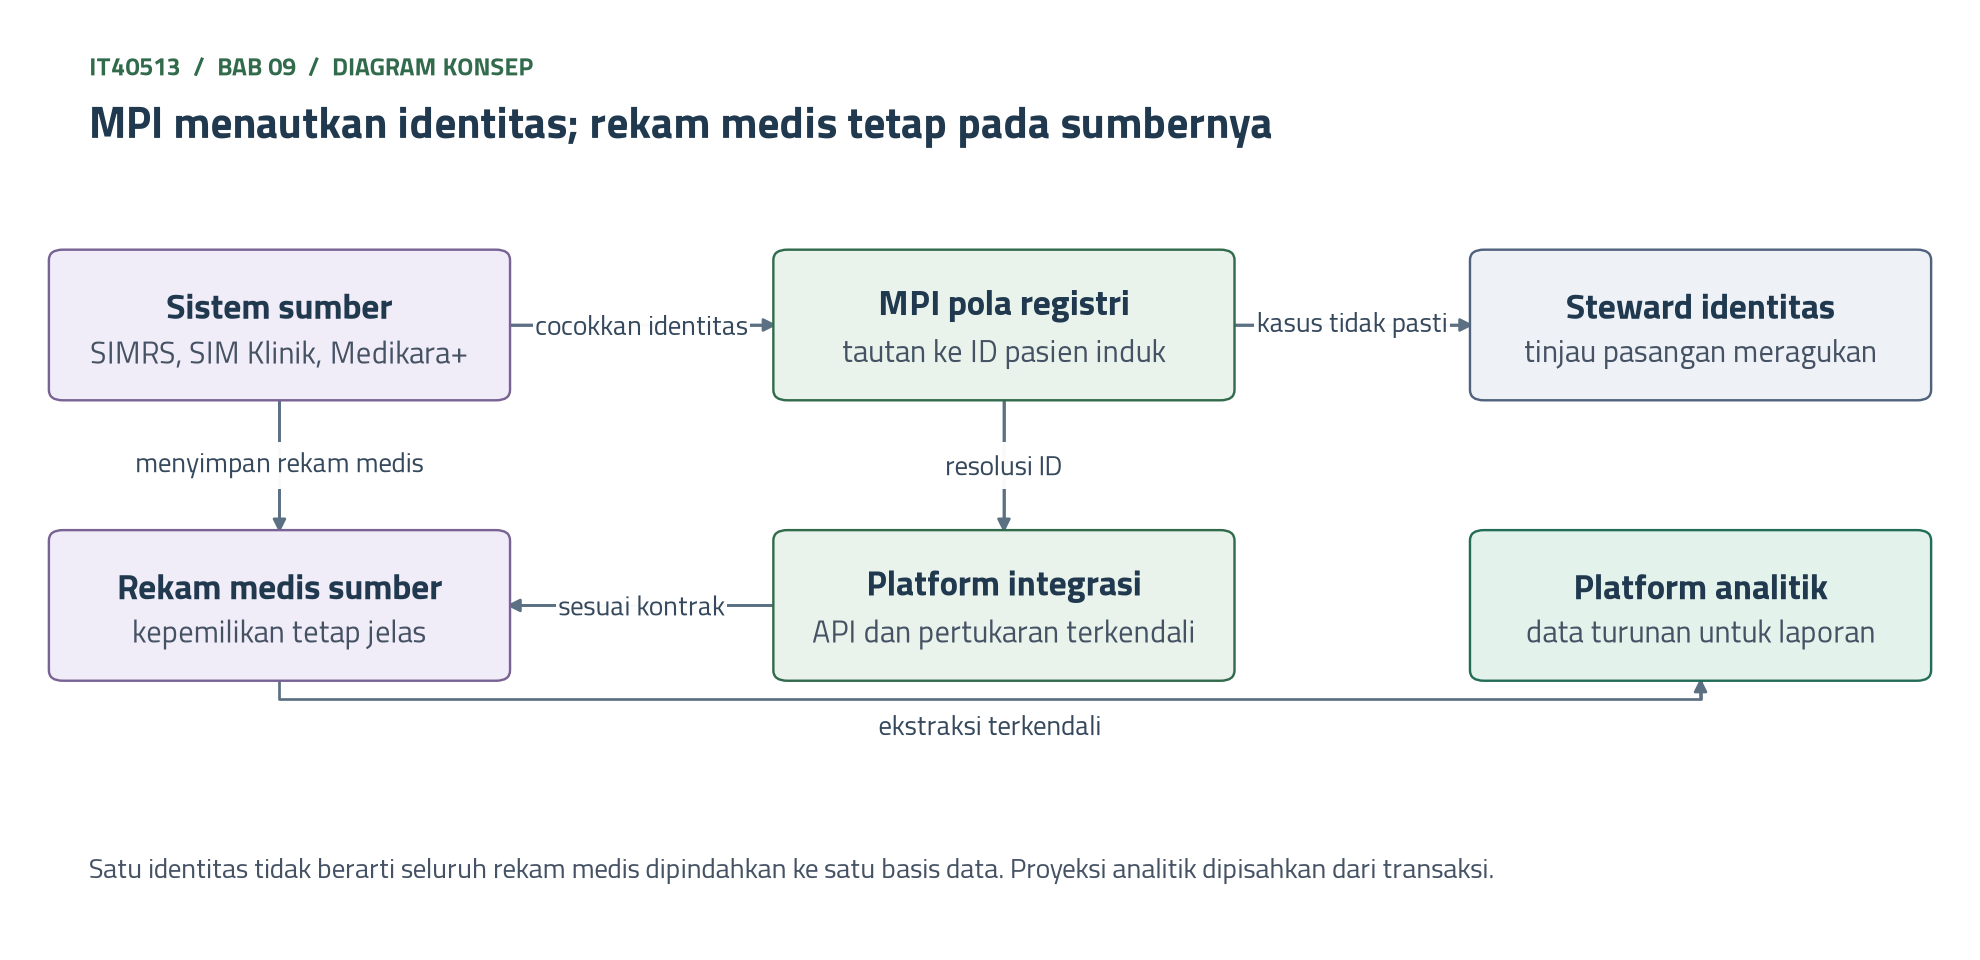
\includegraphics[width=0.96\textwidth,height=0.77\textheight,keepaspectratio]{../../figures/ch09-diagram-konsep.png}
  \label{fig:session09-ilustrasi-bab}
\end{frame}

\begin{frame}{{\Large Master Patient Index}}
  \small
  \vspace{6pt}
  \begin{itemize}
    \item \textit{Master Patient Index} (MPI) menautkan semua nomor lokal milik satu orang ke satu
          identitas induk.
    \item MPI tidak menyimpan rekam medis. Isinya data demografi dan daftar tautan ke nomor lokal.
    \item Saat pasien mendaftar di fasilitas mana pun, aplikasi pendaftaran bertanya ke MPI lebih
          dahulu.
    \item Bila sudah dikenal, MPI mengembalikan ID induk. Bila belum, MPI membuat ID induk baru.
  \end{itemize}
  \vspace{6pt}
  Analogi: buku induk warga di kantor RT. Daftar arisan, ronda, dan posyandu tetap ada, tetapi
  hitungan warga memakai nomor di buku induk.
\end{frame}

\begin{frame}{{\Large Empat Nomor, Satu ID Induk}}
  \centering
  \begin{figure}
    \resizebox{0.88\textwidth}{!}{\begin{tikzpicture}[
  font=\scriptsize,
  kotak/.style={draw, rounded corners, minimum height=0.85cm,
                minimum width=2.5cm, align=center, font=\scriptsize\bfseries},
  panah/.style={-{Stealth[length=2mm]}, thick}
]
  \node[kotak, fill=blue!8] (rsj) at (0,1.8)
    {SIMRS Jakarta\\{\tiny\mdseries nomor 0045812}};
  \node[kotak, fill=blue!8] (rsd) at (0,0.6)
    {SIMRS Depok\\{\tiny\mdseries nomor D-22017}};
  \node[kotak, fill=blue!8] (kln) at (0,-0.6)
    {Klinik Bogor\\{\tiny\mdseries nomor K-118230}};
  \node[kotak, fill=blue!8] (app) at (0,-1.8)
    {Medikara+\\{\tiny\mdseries akun 7731}};

  \node[kotak, fill=praditagreen!15, minimum width=2.9cm,
        minimum height=1.7cm] (mpi) at (4.5,0)
    {MPI Medikara\\[2pt]{\tiny\mdseries ID induk MDK-0318274}\\
     {\tiny\mdseries NIK dan nomor SATUSEHAT}\\
     {\tiny\mdseries empat tautan nomor lokal}};

  \node[kotak, fill=green!10] (rm) at (9,1.2) {Riwayat klinis\\lintas fasilitas};
  \node[kotak, fill=green!10] (lap) at (9,0) {Laporan\\pasien unik};
  \node[kotak, fill=green!10] (ss) at (9,-1.2) {Pengiriman data\\ke SATUSEHAT};

  \draw[panah] (rsj.east) -- ([yshift=0.45cm]mpi.west);
  \draw[panah] (rsd.east) -- ([yshift=0.15cm]mpi.west);
  \draw[panah] (kln.east) -- ([yshift=-0.15cm]mpi.west);
  \draw[panah] (app.east) -- ([yshift=-0.45cm]mpi.west);
  \draw[panah] ([yshift=0.35cm]mpi.east) -- (rm.west);
  \draw[panah] (mpi.east) -- (lap.west);
  \draw[panah] ([yshift=-0.35cm]mpi.east) -- (ss.west);

  \node[font=\tiny, gray, anchor=south] at (0,2.3) {satu orang, empat nomor lokal};
  \node[font=\tiny, gray, anchor=south] at (9,1.75) {satu identitas dipakai ulang};
\end{tikzpicture}
}
    \caption{MPI menautkan empat nomor lokal milik satu pasien ke satu ID induk}
  \end{figure}
\end{frame}

\begin{frame}{{\Large Dua Contoh Dampak Identitas Ganda}}
  \vspace{8pt}
  \begin{itemize}
    \item Misalkan 18.000 pemeriksaan laboratorium per tahun diulang karena hasil fasilitas lain tidak
          terlihat.
    \item Dengan biaya rata-rata Rp150.000, pemborosannya sekitar Rp2.700 juta per tahun.
    \item Laporan direksi 2025 mencatat 150.000 pasien baru.
    \item Setelah dicocokkan, 55.000 di antaranya pasien lama di fasilitas Medikara lain.
    \item Pasien baru yang sesungguhnya sekitar 95.000, atau 36,7 persen lebih sedikit.
  \end{itemize}
\end{frame}

\begin{frame}{{\Large Tiga Pola Manajemen Data Induk}}
  \footnotesize
  \begin{tabularx}{\textwidth}{L{1.8cm}YYL{1.5cm}}
    \hline
    \textbf{Pola} & \textbf{Tempat versi induk} & \textbf{Yang mengubah} & \textbf{Biaya ubah} \\
    \hline
    Registri & Tetap di tiap sistem sumber, pusat hanya menyimpan tautan & Sistem sumber & Rendah \\
    \hline
    Konsolidasi & Salinan bersih di pusat, dipakai untuk dibaca dan dilaporkan & Sistem sumber, pusat merapikan & Sedang \\
    \hline
    Terpusat & Di pusat, sistem sumber membaca dari pusat & Hanya pusat & Tinggi \\
    \hline
  \end{tabularx}

  \vspace{4pt}
  \small
  \begin{itemize}
    \item Data induk obat untuk 12 apotek layak terpusat sejak awal: katalog jarang berubah dan satu
          tim farmasi pusat sudah mengelolanya.
    \item Data induk pasien layak dimulai dari registri: lima SIMRS masih berjalan dan mengubah
          kelimanya mahal.
  \end{itemize}
\end{frame}

\begin{frame}{{\Large Kepemilikan dan Aturan Pembaruan}}
  \footnotesize
  \begin{tabularx}{\textwidth}{L{3.7cm}YY}
    \hline
    \textbf{Atribut} & \textbf{Yang boleh mengubah} & \textbf{Syarat} \\
    \hline
    ID induk & Tidak ada, dibuat otomatis oleh MPI & Tidak pernah dipakai ulang \\
    \hline
    NIK, nama, tanggal lahir & Petugas pendaftaran & Sesuai dokumen identitas yang diperiksa \\
    \hline
    Alamat dan nomor telepon & Petugas pendaftaran, atau pasien lewat Medikara+ & Riwayat perubahan disimpan \\
    \hline
    Nomor SATUSEHAT & Tidak diubah di Medikara & Diambil dari layanan SATUSEHAT \\
    \hline
    Penggabungan dan pemisahan catatan & Tim pengelola data induk & Ditinjau dua orang dan tercatat \\
    \hline
  \end{tabularx}

  \vspace{4pt}
  \small Pemilik bisnis: Direktur Pelayanan. Pengelola harian (\textit{data steward}): kepala
  unit rekam medis tiap fasilitas. Salah gabung adalah kesalahan klinis, sehingga setiap
  penggabungan harus dapat dibatalkan.
\end{frame}

\begin{frame}{{\Large Satu Sumber Kebenaran, Bukan Satu Basis Data}}
  \small
  \vspace{6pt}
  \begin{itemize}
    \item Satu sumber kebenaran: tiap atribut punya satu acuan dan satu jalur resmi untuk mengubahnya.
    \item Satu basis data: semua data disimpan di satu tempat secara fisik.
    \item Pola registri mencapai yang pertama walaupun data masih tersebar di lima SIMRS.
    \item Konsekuensi pertama: aplikasi baru wajib membaca identitas dari MPI dan dilarang membuat
          daftar pasien sendiri.
    \item Konsekuensi kedua: MPI menjadi layanan yang paling sering dipanggil, sehingga
          ketersediaannya menjadi syarat di Bab 10.
  \end{itemize}
\end{frame}

\begin{frame}{{\Large Menyatukan Identitas dalam Dua Tahap}}
  \begin{block}{Kasus Medikara Health}
    \small
    \begin{itemize}
      \item Tahap pertama: MPI berpola registri di atas lima SIMRS, SIM Klinik, dan Medikara+.
      \item Pencocokan awal 2,1 juta catatan menghasilkan sekitar 1,5 juta ID induk.
      \item Misalkan 9.000 pasangan masuk antrean tinjauan. Enam petugas, masing-masing 60 pasangan
            per hari, menyelesaikannya dalam 25 hari kerja.
      \item Tahap kedua: setelah SIMRS tunggal berjalan, MPI berubah menjadi pola terpusat.
      \item MPI Medikara tidak menggantikan MPI nasional Kementerian Kesehatan. Nomor SATUSEHAT
            disimpan sebagai salah satu tautan.
    \end{itemize}
  \end{block}
\end{frame}

\begin{frame}{{\Large Data Operasional dan Data Analitik}}
  \small Misalkan laporan bulanan direksi dirakit dari 23 \textit{spreadsheet} selama sembilan hari
  kerja, dan angka kunjungannya selisih 4 persen.

  \vspace{4pt}
  \footnotesize
  \begin{tabularx}{\textwidth}{L{2.6cm}YY}
    \hline
    \textbf{Hal} & \textbf{Data operasional} & \textbf{Data analitik} \\
    \hline
    Pertanyaan khas & Jam berapa pasien ini dijadwalkan? & Berapa median waktu tunggu tiap rumah sakit selama 12 bulan? \\
    \hline
    Rentang waktu & Saat ini & Bertahun-tahun ke belakang \\
    \hline
    Pola pemakaian & Satu catatan diubah berulang & Banyak catatan dibaca sekaligus \\
    \hline
    Pemakai & Petugas layanan & Manajemen, analis, regulator \\
    \hline
    Bila dicampur & Laporan berat memperlambat pendaftaran & Angka berubah saat laporan sedang dibaca \\
    \hline
  \end{tabularx}

  \vspace{4pt}
  \small Analogi: kasir melayani antrean, bagian pembukuan merekap nota setiap malam.
\end{frame}

\begin{frame}{{\Large Alur Data Target Medikara}}
  \small Gudang data (\textit{data warehouse}), \textit{data lake}, dan \textit{lakehouse} menjawab
  kebutuhan yang sama: satu tempat terkelola untuk data analitik.

  \centering
  \begin{figure}
    \resizebox{0.78\textwidth}{!}{\begin{tikzpicture}[
  font=\scriptsize,
  kotak/.style={draw, rounded corners, minimum height=0.8cm,
                minimum width=1.9cm, align=center, font=\scriptsize\bfseries},
  panah/.style={-{Stealth[length=2mm]}, thick}
]
  \node[kotak, fill=blue!8] (simrs) at (0,1.5) {SIMRS};
  \node[kotak, fill=blue!8] (klinik) at (0,0.5) {SIM Klinik};
  \node[kotak, fill=blue!8] (erp) at (0,-0.5) {ERP keuangan};
  \node[kotak, fill=blue!8] (app) at (0,-1.5) {Medikara+};

  \node[kotak, fill=blue!8, minimum height=1.2cm] (mentah) at (2.45,0)
    {Zona\\mentah\\{\tiny\mdseries salinan apa adanya}};
  \node[kotak, fill=orange!12, minimum height=1.2cm] (mutu) at (4.9,0)
    {Pemeriksaan\\kualitas\\{\tiny\mdseries aturan tertulis}};
  \node[kotak, fill=blue!8, minimum height=1.2cm] (olah) at (7.35,0)
    {Zona\\terolah\\{\tiny\mdseries satu definisi}};
  \node[kotak, fill=praditagreen!15] (mpi) at (7.35,1.75)
    {MPI\\{\tiny\mdseries ID induk pasien}};

  \node[kotak, fill=green!10] (dash) at (9.8,0.6) {\textit{Dashboard}\\direksi};
  \node[kotak, fill=green!10] (reg) at (9.8,-0.6) {Laporan\\eksternal};

  \node[kotak, fill=red!22] (xls) at (4.9,-2.0)
    {Spreadsheet\\manual};

  \foreach \s in {simrs, klinik, erp, app}
    \draw[panah] (\s.east) -- (mentah.west);
  \draw[panah] (mentah) -- (mutu);
  \draw[panah] (mutu) -- (olah);
  \draw[panah] (mpi) -- (olah);
  \draw[panah] (olah.east) -- (dash.west);
  \draw[panah] (olah.east) -- (reg.west);
  \draw[panah, dashed, gray] (xls.east) -| (reg.south);
  \node[font=\tiny, gray, anchor=north] at (7.6,-2.05) {jalur lama, dihentikan bertahap};
  \node[font=\tiny, gray, anchor=south, align=center] at (4.9,0.7)
    {data yang gagal\\dikembalikan ke pemiliknya};
\end{tikzpicture}
}
    \caption{Alur data target untuk analitik dan pelaporan di Medikara}
  \end{figure}
\end{frame}

\begin{frame}{{\Large Satu Definisi untuk Tiap Angka}}
  \small Selisih 4 persen berasal dari dua definisi kunjungan: keuangan menghitung tagihan, pelayanan
  menghitung pendaftaran, termasuk yang batal diperiksa.

  \vspace{4pt}
  \footnotesize
  \begin{tabularx}{\textwidth}{L{2.0cm}YL{2.7cm}}
    \hline
    \textbf{Angka} & \textbf{Definisi tunggal} & \textbf{Pemilik} \\
    \hline
    Kunjungan & Pendaftaran layanan yang berakhir dengan pemeriksaan, dihitung per tanggal layanan & Direktur Pelayanan \\
    \hline
    Pasien unik & Jumlah ID induk MPI dengan minimal satu kunjungan dalam periode & Direktur Pelayanan \\
    \hline
    Waktu tunggu & Selisih jam pendaftaran dan jam mulai pemeriksaan, median per hari & Kepala rawat jalan \\
    \hline
    Klaim tertunda & Klaim BPJS Kesehatan yang belum dibayar lebih dari 30 hari sejak diajukan & Direktur Keuangan \\
    \hline
  \end{tabularx}
\end{frame}

\begin{frame}{{\Large Mengganti Spreadsheet, Menjaga Kualitas}}
  \small
  \vspace{6pt}
  \begin{itemize}
    \item Empat langkah: daftar laporan rutin, bangun ulang dari zona terolah, jalankan paralel dua
          periode, hentikan \textit{spreadsheet} sebagai sumber resmi.
    \item Aturan kualitas dapat dihitung: NIK terisi pada sedikitnya 98 persen pendaftaran baru.
    \item Tanggal pulang tidak pernah lebih awal dari tanggal masuk. Kode diagnosis terisi pada
          sedikitnya 99 persen kunjungan yang sudah ditutup.
    \item Target pertama: laporan bulanan tersedia dua hari kerja setelah bulan berakhir, turun dari
          sembilan hari kerja.
    \item Target kedua: kelengkapan NIK naik dari 77,4 persen pada data lama menjadi 98 persen pada
          pendaftaran baru.
  \end{itemize}
\end{frame}

\section{Lanskap Aplikasi dan Integrasi}

\begin{frame}{\hfill}
  \centering
  \Huge{\textbf{Lanskap Aplikasi\\dan Integrasi}}
\end{frame}

\begin{frame}{{\Large Empat Keputusan Rasionalisasi}}
  \small Misalkan katalog Bab 7 mencatat 46 aplikasi. Aplikasi tanpa keputusan tetap berjalan, tetap
  dibayar, dan tetap menjadi celah keamanan.

  \vspace{4pt}
  \footnotesize
  \begin{tabularx}{\textwidth}{L{2.1cm}YL{3.0cm}}
    \hline
    \textbf{Keputusan} & \textbf{Artinya} & \textbf{TIME yang lazim} \\
    \hline
    Pertahankan & Aplikasi tetap dipakai di kondisi target, mungkin dengan perbaikan & \textit{Invest}, \textit{Tolerate} \\
    \hline
    Ganti & Fungsinya tetap dibutuhkan, tetapi aplikasinya diganti & \textit{Migrate} \\
    \hline
    Gabungkan & Beberapa aplikasi sefungsi disatukan menjadi satu & \textit{Tolerate}, \textit{Migrate} \\
    \hline
    Hentikan & Fungsinya tidak lagi dibutuhkan atau sudah dilayani aplikasi lain & \textit{Eliminate} \\
    \hline
  \end{tabularx}

  \vspace{4pt}
  \small Analogi: membereskan dapur setelah dua keluarga pindah serumah. Barang tidak disumbangkan
  sebelum dipastikan tidak ada yang masih memakainya.
\end{frame}

\begin{frame}{{\Large TIME, Rasionalisasi, dan Aplikasi Bersama}}
  \small
  \vspace{6pt}
  \begin{itemize}
    \item TIME (\textit{Tolerate, Invest, Migrate, Eliminate}) menilai kondisi aplikasi saat ini dari
          nilai bisnis dan kualitas teknis.
    \item Rasionalisasi memutuskan nasib aplikasi di kondisi target: kapabilitas, prinsip arsitektur,
          dan aplikasi lain yang fungsinya sama.
    \item Kapabilitas yang distandarkan memakai aplikasi bersama, bagian dari \textit{operational
          backbone}.
    \item Aplikasi lokal boleh bila membaca identitas dari MPI dan terhubung lewat platform integrasi.
    \item Antrean Bandung dihentikan setelah data dua tahun dipindahkan. SIM Klinik digabungkan ke
          SIMRS tunggal.
  \end{itemize}
\end{frame}

\begin{frame}{{\Large Lanskap Aplikasi Target}}
  \centering
  \begin{figure}
    \resizebox{0.84\textwidth}{!}{\begin{tikzpicture}[
  font=\scriptsize,
  kotak/.style={draw, rounded corners, minimum height=0.8cm,
                minimum width=1.8cm, align=center, font=\scriptsize\bfseries},
  panah/.style={-{Stealth[length=2mm]}, thick},
  garis/.style={thick}
]
  % Kanal
  \node[kotak, fill=blue!8, minimum width=2.6cm] (medi) at (2.0,2.6)
    {Medikara+\\{\tiny\mdseries pasien}};
  \node[kotak, fill=orange!12, minimum width=2.6cm] (mitra) at (6.1,2.6)
    {Portal mitra\\{\tiny\mdseries klinik mitra, asuransi}};

  % Platform integrasi
  \node[kotak, fill=orange!12, minimum width=8.1cm, minimum height=0.7cm]
    (integ) at (4.05,1.3) {Platform integrasi dan \textit{API gateway}};

  % Aplikasi inti bersama
  \node[kotak, fill=blue!8] (simrs) at (0.9,0)
    {SIMRS tunggal\\{\tiny\mdseries 5 rumah sakit, 18 klinik}};
  \node[kotak, fill=blue!8] (erp) at (3.0,0)
    {ERP\\{\tiny\mdseries keuangan}};
  \node[kotak, fill=praditagreen!15] (mpi) at (5.1,0)
    {MPI\\{\tiny\mdseries data induk pasien}};
  \node[kotak, fill=blue!8] (lis) at (7.2,0)
    {Sistem lab\\dan apotek};

  % Platform data
  \node[kotak, fill=green!10, minimum width=8.1cm, minimum height=0.7cm]
    (data) at (4.05,-1.3) {Platform data analitik dan \textit{dashboard} manajemen};

  % Pihak eksternal
  \node[kotak, fill=white, dashed, minimum width=1.9cm] (ss) at (10.1,1.9)
    {SATUSEHAT\\{\tiny\mdseries FHIR R4}};
  \node[kotak, fill=white, dashed, minimum width=1.9cm] (bpjs) at (10.1,0.7)
    {BPJS\\Kesehatan};

  \draw[panah] (medi) -- (medi |- integ.north);
  \draw[panah] (mitra) -- (mitra |- integ.north);
  \foreach \apl in {simrs, erp, mpi, lis} {
    \draw[garis] (\apl.north) -- (\apl |- integ.south);
    \draw[panah] (\apl.south) -- (\apl |- data.north);
  }
  \draw[panah] (integ.east) -- ++(0.35,0) |- (ss.west);
  \draw[panah] (integ.east) -- ++(0.35,0) |- (bpjs.west);

  \node[font=\tiny, gray, anchor=north] at (10.1,0.15)
    {pihak eksternal};
\end{tikzpicture}
}
    \caption{Lanskap aplikasi target Medikara: kanal, platform integrasi, aplikasi inti bersama, dan platform data}
  \end{figure}
\end{frame}

\begin{frame}{{\Large Rasionalisasi Aplikasi Medikara}}
  \begin{block}{Kasus Medikara Health}
    \scriptsize
    \begin{tabularx}{\linewidth}{L{3.4cm}L{1.5cm}Y}
      \hline
      \textbf{Aplikasi saat ini} & \textbf{Keputusan} & \textbf{Alasan singkat} \\
      \hline
      Lima SIMRS & Ganti & Lima versi hasil akuisisi diganti satu SIMRS tunggal (\textit{Migrate}) \\
      \hline
      SIM Klinik & Gabungkan & Modul rawat jalan SIMRS tunggal melayani 18 klinik (\textit{Tolerate}) \\
      \hline
      ERP keuangan & Pertahankan & Sudah terpusat, ditambah antarmuka tagihan dan klaim (\textit{Invest}) \\
      \hline
      Medikara+ & Pertahankan & Kanal pasien utama, akses datanya dipindah ke API (\textit{Invest}) \\
      \hline
      Antrean rumah sakit Bandung & Hentikan & Fungsinya sudah ada di Medikara+ (\textit{Eliminate}) \\
      \hline
      23 \textit{spreadsheet} laporan & Hentikan & Diganti laporan dari platform data (\textit{Eliminate}) \\
      \hline
      Integrasi ke BPJS dan SATUSEHAT & Ganti & Dipindah ke platform integrasi (\textit{Migrate}) \\
      \hline
    \end{tabularx}

    \vspace{4pt}
    \footnotesize Medikara+ tidak lagi membaca basis data SIMRS secara langsung, melainkan lewat API
    yang hak aksesnya dibatasi. ERP tetap menjadi satu-satunya sumber data keuangan.
  \end{block}
\end{frame}

\begin{frame}{{\Large Enam Pemeriksaan sebelum Aplikasi Dihentikan}}
  \scriptsize
  \begin{tabularx}{\textwidth}{L{2.1cm}YY}
    \hline
    \textbf{Pemeriksaan} & \textbf{Pertanyaan} & \textbf{Bukti yang dicari} \\
    \hline
    Pengguna & Siapa yang masih masuk ke aplikasi dalam 90 hari terakhir? & Log akses \\
    \hline
    Keluaran wajib & Laporan apa yang masih dihasilkan, dan dikirim ke mana? & Daftar laporan dan jadwal pengirimannya \\
    \hline
    Data & Data apa yang wajib disimpan, dan di mana diarsipkan? & Aturan penyimpanan dan rencana arsip \\
    \hline
    Ketergantungan & Integrasi atau proses apa yang membaca dari aplikasi ini? & Katalog antarmuka Bab 7 \\
    \hline
    Kontrak & Kapan kontrak berakhir, dan bagaimana data dikembalikan? & Kontrak vendor \\
    \hline
    Pengganti & Apakah fungsi pengganti sudah diuji paralel? & Hasil uji dan persetujuan pemilik \\
    \hline
  \end{tabularx}

  \vspace{6pt}
  \small Permenkes 24/2022 Pasal 20 menuntut penyimpanan yang aman, utuh, rahasia, dan tersedia.
  Rencana arsip harus siap sebelum tanggal penghentian ditetapkan.
\end{frame}

\begin{frame}{{\Large Hub, Platform Integrasi, dan API}}
  \small
  \vspace{6pt}
  \begin{itemize}
    \item Sembilan sistem pada Bab 7 dapat membentuk paling banyak 36 koneksi \textit{point-to-point}.
    \item \textit{Hub}: perantara tunggal. Tiap aplikasi cukup terhubung ke \textit{hub}.
    \item Platform integrasi: \textit{hub} dengan penerjemahan format, antrean pesan, pemantauan, dan
          pencatatan pertukaran.
    \item API (\textit{Application Programming Interface}): kontrak antarmuka tentang data apa, format
          apa, dan oleh siapa.
  \end{itemize}
  \vspace{6pt}
  Analogi: sembilan kota dengan satu terminal bus pusat. Bila terminal tutup, semua perjalanan
  berhenti, sehingga terminal dijaga paling ketat.
\end{frame}

\begin{frame}{{\Large Dari Point-to-Point ke Hub}}
  \centering
  \begin{figure}
    \resizebox{0.68\textwidth}{!}{\begin{tikzpicture}[
  font=\scriptsize,
  simpul/.style={draw, rounded corners, minimum height=0.5cm,
                 minimum width=1.5cm, align=center, font=\scriptsize\bfseries},
  garis/.style={thick, gray}
]
  % Kiri: point-to-point, enam aplikasi saling terhubung langsung
  \foreach \nama [count=\i] in {SIMRS, SIM Klinik, ERP, Medikara+, SATUSEHAT, BPJS} {
    \node[simpul, fill=blue!8] (p\i) at ({90-60*(\i-1)}:1.8) {\nama};
  }
  \begin{scope}[on background layer]
    \foreach \i in {1,...,6} {
      \foreach \j in {1,...,6} {
        \ifnum\i<\j
          \draw[garis, red!45] (p\i) -- (p\j);
        \fi
      }
    }
  \end{scope}
  \node[font=\scriptsize\bfseries, anchor=north] at (0,-2.35)
    {\textit{Point-to-point}: 15 koneksi};

  % Kanan: hub, tiap aplikasi cukup satu koneksi
  \node[simpul, fill=orange!12, minimum width=1.7cm, minimum height=0.9cm]
    (hub) at (6.9,0) {Platform\\integrasi};
  \foreach \nama [count=\i] in {SIMRS, SIM Klinik, ERP, Medikara+, SATUSEHAT, BPJS} {
    \node[simpul, fill=blue!8] (h\i) at ($(hub)+({90-60*(\i-1)}:1.8)$) {\nama};
    \begin{scope}[on background layer]
      \draw[garis, praditagreen] (hub) -- (h\i);
    \end{scope}
  }
  \node[font=\scriptsize\bfseries, anchor=north] at (6.9,-2.35)
    {\textit{Hub}: 6 koneksi};
\end{tikzpicture}
}
    \caption{Koneksi \textit{point-to-point} dibandingkan dengan \textit{hub} untuk enam aplikasi}
  \end{figure}
  \vspace{-4pt}
  \small Untuk sembilan sistem, batas model 36 koneksi menjadi 9; keadaan nyata pada Bab 7 adalah 21
  pasangan aktif. Platform integrasi menjadi titik tunggal yang harus tersedia tinggi.
\end{frame}

\begin{frame}{{\Large Integrasi Target dan Pihak Eksternal}}
  \scriptsize
  \begin{tabularx}{\textwidth}{L{2.2cm}L{2.2cm}YL{3.2cm}}
    \hline
    \textbf{Dari} & \textbf{Ke} & \textbf{Data} & \textbf{Gaya} \\
    \hline
    SIMRS tunggal & MPI & Identitas pasien & Permintaan dan jawaban \\
    \hline
    SIMRS tunggal & SATUSEHAT & Kunjungan, diagnosis, hasil pemeriksaan & Pesan, format FHIR R4 \\
    \hline
    SIMRS tunggal & BPJS Kesehatan & Data klaim & Permintaan dan jawaban \\
    \hline
    SIMRS tunggal & ERP keuangan & Tagihan final & Pesan \\
    \hline
    Medikara+ & SIMRS tunggal & Jadwal dan janji temu & Permintaan dan jawaban \\
    \hline
    Aplikasi inti & Platform data & Transaksi harian & Salinan terjadwal \\
    \hline
  \end{tabularx}

  \vspace{6pt}
  \small Satu penghubung untuk tiap pihak eksternal di platform integrasi, bukan di tiap SIMRS.
  Permenkes 24/2022 Pasal 21 mewajibkan rekam medis elektronik terhubung dengan platform yang dikelola
  Kementerian Kesehatan, yaitu SATUSEHAT. Rincian API dibahas di IT40613.
\end{frame}

\section{Membangun, Membeli, Berlangganan}

\begin{frame}{\hfill}
  \centering
  \Huge{\textbf{Membangun, Membeli,\\atau Berlangganan}}
\end{frame}

\begin{frame}{{\Large Tiga Cara Memperoleh Aplikasi}}
  \footnotesize
  \begin{tabularx}{\textwidth}{L{3.1cm}YYY}
    \hline
    \textbf{Hal} & \textbf{Membangun} & \textbf{Membeli} & \textbf{Berlangganan SaaS} \\
    \hline
    Kesesuaian proses & Paling tinggi & Sedang, lewat konfigurasi & Mengikuti produk \\
    \hline
    Biaya awal & Tinggi & Sedang sampai tinggi & Rendah \\
    \hline
    Waktu sampai dipakai & Paling lama & Sedang & Paling cepat \\
    \hline
    Kendali atas data & Penuh & Penuh & Ditentukan kontrak \\
    \hline
    Ketergantungan & Pada tim sendiri & Pada vendor, sedang & Pada penyedia, tinggi \\
    \hline
    Tanggung jawab keamanan & Organisasi seluruhnya & Organisasi, dibantu vendor & Dibagi dengan penyedia \\
    \hline
  \end{tabularx}

  \vspace{6pt}
  \small Analogi: membangun rumah sendiri, membeli rumah jadi, atau menyewa apartemen.
\end{frame}

\begin{frame}{{\Large Lima Kriteria sebelum Vendor Dinilai}}
  \small
  \vspace{4pt}
  \begin{itemize}
    \item Kesesuaian kapabilitas: kapabilitas target Bab 8 yang didukung tanpa kustomisasi berat.
    \item Biaya total lima tahun: lisensi atau langganan, implementasi, migrasi data, operasi, dan
          pelatihan.
    \item Waktu sampai bernilai: kapan lima rumah sakit dan 18 klinik benar-benar memakainya.
    \item Ketergantungan vendor: kemudahan mengambil data saat kontrak berakhir dan dukungan pada
          standar terbuka seperti FHIR.
    \item Kepatuhan: Permenkes 24/2022 Pasal 20 ayat (3) membatasi media penyimpanan, Pasal 22
          mensyaratkan fasilitas penyimpanan mitra di dalam negeri.
  \end{itemize}
\end{frame}

\begin{frame}{{\Large Matriks Berbobot dan Uji Sensitivitas}}
  \footnotesize
  \begin{tabularx}{\textwidth}{Xrrrr}
    \hline
    \textbf{Kriteria (angka rekaan)} & \textbf{Bobot} & \textbf{Membangun} & \textbf{Membeli} & \textbf{SaaS} \\
    \hline
    Kesesuaian kapabilitas & 30 & 4 & 4 & 3 \\
    \hline
    Biaya total lima tahun & 25 & 2 & 3 & 4 \\
    \hline
    Waktu sampai bernilai & 15 & 1 & 3 & 5 \\
    \hline
    Ketergantungan vendor & 15 & 5 & 3 & 2 \\
    \hline
    Kepatuhan & 15 & 4 & 4 & 3 \\
    \hline
    \textbf{Skor berbobot} & \textbf{100} & \textbf{3,20} & \textbf{3,45} & \textbf{3,40} \\
    \hline
  \end{tabularx}

  \vspace{6pt}
  \begin{tabularx}{\textwidth}{Xrrrl}
    \hline
    \textbf{Skenario bobot} & \textbf{Bangun} & \textbf{Beli} & \textbf{SaaS} & \textbf{Unggul} \\
    \hline
    Kepatuhan diutamakan: 30, 25, 10, 15, 20 & 3,35 & 3,50 & 3,30 & Beli \\
    \hline
    Kecepatan diutamakan: 20, 25, 25, 15, 15 & 2,90 & 3,35 & 3,60 & SaaS \\
    \hline
  \end{tabularx}

  \vspace{6pt}
  \small Selisih 0,05 terlalu kecil untuk menjadi satu-satunya dasar. Yang perlu disepakati direksi
  lebih dahulu adalah bobotnya, bukan opsinya.
\end{frame}

\begin{frame}{{\Large Risiko Pihak Ketiga dan Catatan Keputusan}}
  \small
  \vspace{6pt}
  \begin{itemize}
    \item Lewat jalur mana vendor menyentuh data: API dengan hak akses sempit, atau akses langsung ke
          basis data?
    \item Data apa yang keluar dari Medikara, dan di mana disimpan?
    \item Bagaimana data diambil kembali dan dimusnahkan di sisi vendor ketika kontrak berakhir?
    \item Apakah vendor mendukung standar terbuka sehingga penggantinya tidak mulai dari nol?
    \item Keputusan besar ditulis sebagai catatan, termasuk syarat peninjauan ulangnya. Format bakunya
          dibahas di Bab 10.
  \end{itemize}
\end{frame}

\begin{frame}{{\Large Pelajaran dari Insiden 2025}}
  \begin{block}{Kasus Medikara Health}
    \small
    Misalkan penelusuran insiden kebocoran data lewat vendor menemukan tiga hal:
    \begin{itemize}
      \item Akun dukungan vendor yang masih aktif memanggil API bawaan dua SIMRS: 8 malam, 1.240 rekam.
      \item Salinan data pengujian disimpan di server vendor tanpa disamarkan.
      \item Kontrak tidak mengatur pengembalian dan pemusnahan data.
    \end{itemize}
    \vspace{4pt}
    Aturan target: vendor hanya lewat platform integrasi dan API berhak akses sempit, data pengujian
    wajib disamarkan, dan rencana keluar menjadi syarat kontrak.
  \end{block}
\end{frame}

\section{Aktivitas dan Penutup}

\begin{frame}{\hfill}
  \centering
  \Huge{\textbf{Aktivitas dan Penutup}}
\end{frame}

\begin{frame}{{\Large Aktivitas: Data dan Aplikasi Target}}
  \small
  \begin{itemize}
    \item Rancang identitas tunggal: atribut, pola data induk, pemilik, dan aturan pembaruan.
    \item Pilih tiga laporan terpenting, tulis definisi tunggal tiap angka, lalu gambar alur datanya.
    \item Isi tabel rasionalisasi untuk setiap aplikasi di katalog C2.
    \item Bandingkan minimal dua opsi dengan kriteria berbobot, lalu uji skenario bobot lain.
    \item Susun tabel integrasi target, selaraskan dengan tim IT40613, lalu modelkan di Archi.
  \end{itemize}
  \footnotesize Peran: analis teknologi, analis bisnis, pemodel, koordinator. Luaran: tonggak C3.
  Penilaian: keterlacakan 30, tabel rasionalisasi 25, matriks 25, model 20 persen.
  Lembar kerja: \berkas{sources/chapter09/lembar-kerja-aktivitas.md}.
\end{frame}

\begin{frame}{{\Large Ringkasan}}
  \small
  \vspace{6pt}
  \begin{itemize}
    \item Sebanyak 2,1 juta catatan mewakili sekitar 1,5 juta orang. Arsitektur data dimulai dari
          identitas, bukan dari \textit{dashboard}.
    \item MPI menautkan nomor lokal ke satu ID induk. Medikara mulai dari registri, lalu terpusat.
    \item Data analitik mengalir lewat zona mentah, pemeriksaan kualitas, dan zona terolah.
    \item Tiap aplikasi mendapat satu keputusan. Integrasi berpindah dari 21 pasangan aktif, dengan batas
          model 36, ke 9 koneksi.
    \item Keputusan harus dapat ditelusuri ke kapabilitas dan prinsip. Bobot disepakati lebih dahulu
          daripada pilihan vendor.
  \end{itemize}
\end{frame}

\begin{frame}{{\Large Latihan}}
  \small
  \vspace{6pt}
  \begin{itemize}
    \item \textbf{Latihan 1: Menjelaskan MPI kepada Direksi.} Hitung angka laporan per nomor dan per
          orang, lalu tulis penjelasan paling banyak 150 kata tanpa istilah teknis.
    \item \textbf{Latihan 2: Kriteria Membangun atau Membeli SIMRS.} Susun lima kriteria, bobot total
          100, skor 1 sampai 5, dan satu skenario bobot lain.
    \item \textbf{Latihan 3: Memeriksa Aplikasi Eliminate sebelum Dihentikan.} Telusuri pengguna,
          laporan ke regulator, data, dan kontrak, lalu rancang uji paralel.
  \end{itemize}
  \vspace{6pt}
  Hasil tiap mahasiswa boleh berbeda. Yang dinilai adalah penalaran dan perbandingannya.
\end{frame}

\begin{frame}{{\Large Bacaan dan Berkas Pendukung}}
  \small
  \vspace{6pt}
  \begin{itemize}
    \item \href{https://www.opengroup.org/togaf}{The TOGAF Standard, 10th Edition (2025 Update)}
    \item \href{https://dama.org/articles/introducing-the-revised-dama-data-management-body-of-knowledge-2nd-edition}{DAMA-DMBOK: Data Management Body of Knowledge}
    \item \href{https://peraturan.bpk.go.id/Details/245544}{Peraturan Menteri Kesehatan Nomor 24 Tahun 2022 tentang Rekam Medis}
    \item \berkas{sources/chapter09/README.md}
  \end{itemize}
\end{frame}

\end{document}
